\section{Fast project}

The full code of the \texttt{Android} application is available on this \texttt{GitHub} repository:
\href{https://github.com/LucaLand/MobileSystemsProject-LL/tree/0.9.1/app/src/main/java/it/unibo/mobilesystems}{\textit{link}}.\\
The full code of the \texttt{kBluez} library is available on this \texttt{GitHub} repository: \href{https://github.com/LM-96/MobileSystemProject/tree/main/kBluez/lib/src/main/kotlin/it/unibo/kBluez}{link}.

\subsection{Project of the \texttt{Bluetooth} communications}

As said in the fast analysis, \texttt{Bluetooth} is the chosen communication technology to realize the interaction between robot and user's device.
Android developer documentation fully explain how to set up \href{https://developer.android.com/guide/topics/connectivity/bluetooth}{\texttt{Bluetooth}} while \href{https://github.com/LM-96/MobileSystemProject/tree/main/kBluez}{\texttt{kBluez}} is made by us to make this project work.

About \texttt{Android}, as suggested by the documentation, the main operation to \textit{connect} to a device is:
\begin{itemize}
	\item \textbf{find} the device by executing a \textit{discovery} operation;
	\item \textbf{connect} to the discovered device obtaining a \href{https://developer.android.com/reference/android/bluetooth/BluetoothSocket}{\texttt{BluetoothSocket}};
	\item \textbf{exchange} data throw the socket.
\end{itemize}
\textbf{Notice that differently from the normal \textit{INET} socket, the \texttt{Bluetooth} connection can be established only using the \texttt{UUID} of a \href{https://en.wikipedia.org/wiki/List_of_Bluetooth_protocols\#Radio_frequency_communication_(RFCOMM)}{\texttt{RFCOMM}} service}.

In addition to this, in \texttt{Android} some operations are natively realized with some asynchronous mechanism such as \href{https://developer.android.com/reference/android/content/IntentFilter}{\texttt{IntentFilter}} or \href{https://developer.android.com/reference/android/content/BroadcastReceiver}{\texttt{BroadcastReceiver}}. The obvious motivation for that is to prevent some \textit{unconscious} use of blocking \texttt{IO} operations on the main thread that with this mechanism is avoided.

Even if this way \textit{to do the things} should more safe, it introduces some complications especially for the legibility of code: indeed the developer must register \textit{receiver} that will be activated when required the action has been performed, like imposed by \texttt{Intent} or \texttt{BroadcastReceiver}.

Then, consider if you want to perform a discovery operation using bluetooth in order to search for devices, storing the results in a collection. Following the android guide, the developer must use this pattern:

\begin{lstlisting}[language=Kotlin]
//The collection to store results
val devices = ConcurrentLinkedDeque<BluetoothDevice>()
	
override fun onCreate(savedInstanceState: Bundle?) {
	...
	
	// Register for broadcasts when a device is discovered.
	val filter = IntentFilter(BluetoothDevice.ACTION_FOUND)
	registerReceiver(receiver, filter)
	
	//Start the discovery
	bluetoothAdapter.startDiscovery()
}

// Create a BroadcastReceiver for ACTION_FOUND.
private val receiver = object : BroadcastReceiver() {
	
	override fun onReceive(context: Context, intent: Intent) {
		val action: String = intent.action
		when(action) {
			BluetoothDevice.ACTION_FOUND -> {
				// Discovery has found a device. Get the BluetoothDevice
				// object and its info from the Intent.
				val device: BluetoothDevice =
				intent.getParcelableExtra(BluetoothDevice.EXTRA_DEVICE)
				devices.add(device)
			}
		}
	}
}

override fun onDestroy() {
	super.onDestroy()
	...
	
	// Don't forget to unregister the ACTION_FOUND receiver.
	unregisterReceiver(receiver)
}
\end{lstlisting}

We could make this code more \textit{elegant} using the smart notation of \texttt{Kotlin} lambdas, but however asynchronism could confuse the developer. In addition to this, if the operation are nested (for example, \textit{if a device is found that connect to it}) then code inevitably ends with a \textit{storm} of lambdas which can be very illegible.

For this reason, we decide to provide a solution that restore the synchronism by using the simple class \href{https://github.com/LucaLand/MobileSystemsProject-LL/blob/0.9.1/app/src/main/java/it/unibo/mobilesystems/bluetooth/BluetoothDiscoveryBroadcastReceiver.kt}{\texttt{BluetoothDiscoveryBroadcastReceiver}} and coroutines:
\begin{lstlisting}[language=Kotlin]
private val resultChan = Channel<Any>()
private val bluetoothDiscoveryBroadcastReceiver =
						BluetoothDiscoveryBroadcastReceiver()
private val controllerOnDeviceDiscovered : (BluetoothDevice) -> Unit =
{ device ->
	scope.launch {resultChan.send(device)}
}
private val controllerOnDiscoveryFinished : () -> Unit =
{
	scope.launch {resultChan.send(BluetoothAdapter.ACTION_DISCOVERY_FINISHED)}
}
	
suspend fun discoverDevice(activity : Activity,
							onDeviceDiscovered : (BluetoothDevice) -> Unit = {}) :
									Set<BluetoothDevice> {
	bluetoothDiscoveryBroadcastReceiver
				.addOnDeviceDiscovered(onDeviceDiscovered)
	bluetoothDiscoveryBroadcastReceiver
				.addOnDeviceDiscovered(controllerOnDeviceDiscovered)
	bluetoothDiscoveryBroadcastReceiver
				.addOnDiscoveryFinished(controllerOnDiscoveryFinished)
	
	withContext(Dispatchers.Main) {
		val actionFoundFilter = IntentFilter(BluetoothDevice.ACTION_FOUND)
		activity.registerReceiver(bluetoothDiscoveryBroadcastReceiver,
									actionFoundFilter)
		val discoveryFinishedFilter = IntentFilter(
								BluetoothAdapter.ACTION_DISCOVERY_FINISHED)
		activity.registerReceiver(bluetoothDiscoveryBroadcastReceiver,
									discoveryFinishedFilter)
		bluetoothAdapter!!.startDiscovery()
	}

	val devices = mutableSetOf<BluetoothDevice>()
	var res : Any
	do {
		res = resultChan.receive()
		when(res) {
			is BluetoothDevice -> {
				devices.add(res)
			}
		}
	} while (!(res is String &&
					res == BluetoothAdapter.ACTION_DISCOVERY_FINISHED))

	withContext(Dispatchers.Main) {
		activity.unregisterReceiver(bluetoothDiscoveryBroadcastReceiver)
	}
	bluetoothDiscoveryBroadcastReceiver
				.removeOnDeviceDiscovered(onDeviceDiscovered)
	bluetoothDiscoveryBroadcastReceiver
				.removeOnDeviceDiscovered(controllerOnDeviceDiscovered)
	bluetoothDiscoveryBroadcastReceiver
				.removeOnDiscoveryFinished(controllerOnDiscoveryFinished)

	return devices
}
\end{lstlisting}

\textbf{Notice thatn\texttt{discoverDevice} is a method that is executed by a coroutine that waits for the discovery operation completion.} Theoretically, this method should introduce only a very small overhead caused by the \texttt{scope.launch} that is present by the lambda that are invoked from the \texttt{BroadcastReceiver} of the bluetooth. Indeed, the suspension of calling coroutine on the result channel should introduce no additional costs.

In future implementations, this function might be refined in order to be called also from coroutines that are executing on the main thread by using the appropriate dispatcher.

\begin{figure}[h!]
	\centering
	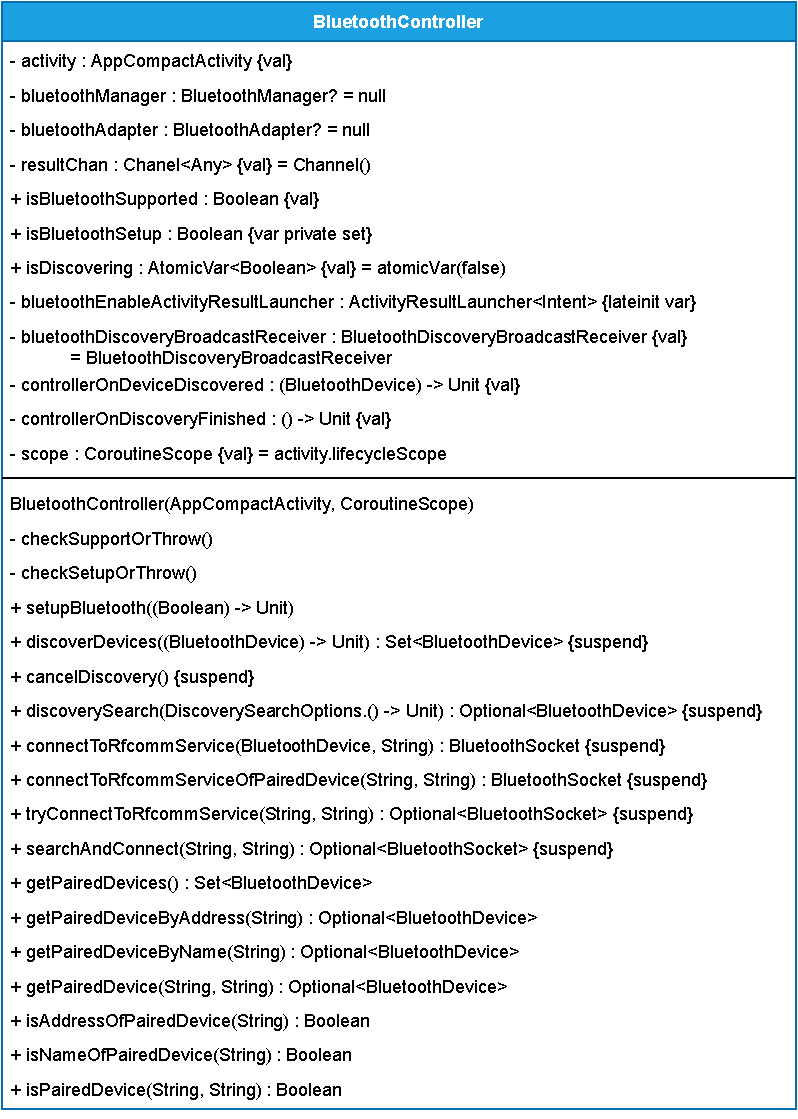
\includegraphics[width=0.7\textwidth]{img/bluetoothcontroller_uml.pdf}
	\caption{UML diagram of \texttt{BluetoothController}}
	\label{fig:bluetoothcontroller_uml}
\end{figure}

Other Bluetooth operations also use this pattern so the figure \ref{fig:bluetoothcontroller_uml} shows the \texttt{UML} diagram of a \textit{controller} for the Bluetooth that can be used from \texttt{BluetoothActivity}.

\begin{figure}[h!]
	\centering
	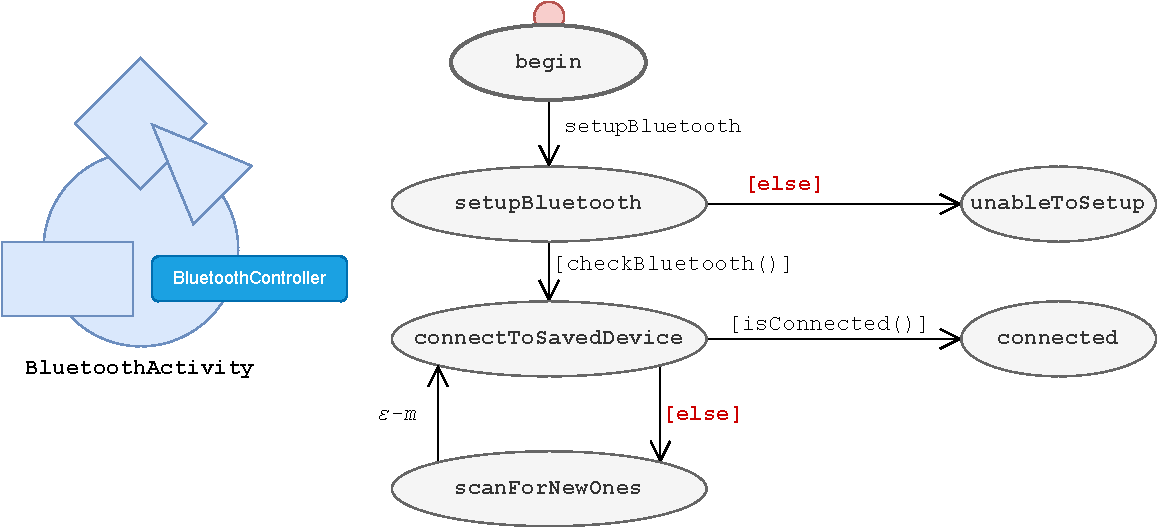
\includegraphics[width=\textwidth]{img/bluetoothactivity.pdf}
	\caption{State diagram of \texttt{BluetoothActivity}}
	\label{fig:bluetoothactivity}
\end{figure}

The figure \ref{fig:bluetoothactivity} shows the state diagram of the \href{https://github.com/LucaLand/MobileSystemsProject-LL/blob/0.9.1/app/src/main/java/it/unibo/mobilesystems/BluetoothConnectionActivity.kt}{\texttt{BluetoothActivity}}. Notice that \textbf{the method \texttt{setupBluetooth} of the controller must be called into the \texttt{onCreate} method of \texttt{Activity} in order to make it work}.

About the states in \texttt{BluetoothActivity}:
\begin{itemize}
	\item \textbf{begin}:\\
	in this state the actor prepare itself for doing the Bluetooth operations and showing results.
	
	\item \textbf{setupBluetooth}:\\
	the actor check if Bluetooth is already been set up by the activity: if not, the actor goes into \textbf{unableToSetupStatus} that only shows to the user a toast saying that it is not possible to use Bluetooth.
	
	\item \textbf{connectToSavedDevice}:\\
	the actor tries to connect the \textit{saved device} that is the last correctly used by the application.
	
	\item \textbf{scanForNewOnes}:\\
	the actor uses the controller to scan for devices showing the found in real time. When the user selects a device, the actor immediately transit to \textbf{connectToSavedDevice} by epsilon move.
	
\end{itemize}
\textbf{We also underline that the actor waits for a \texttt{setupBluetooth} message from its activity in order to perform Bluetooth operations}: this allows to set up Bluetooth from the \texttt{onCreate}, notifying the actor when this operation is concluded, so the actor can correctly use a well initiated controller. 

\subsection{Project of \texttt{GATT} functionalities}

As said in the fast analysis, we have to implement a mechanism based on \texttt{GATT} protocol in order to make the robot able to be stopped by the business logic when it is far from the user.

For this reason, in the logical architecture the analyst has inserted a \texttt{GattActor}.

\begin{figure}[h!]
	\centering
	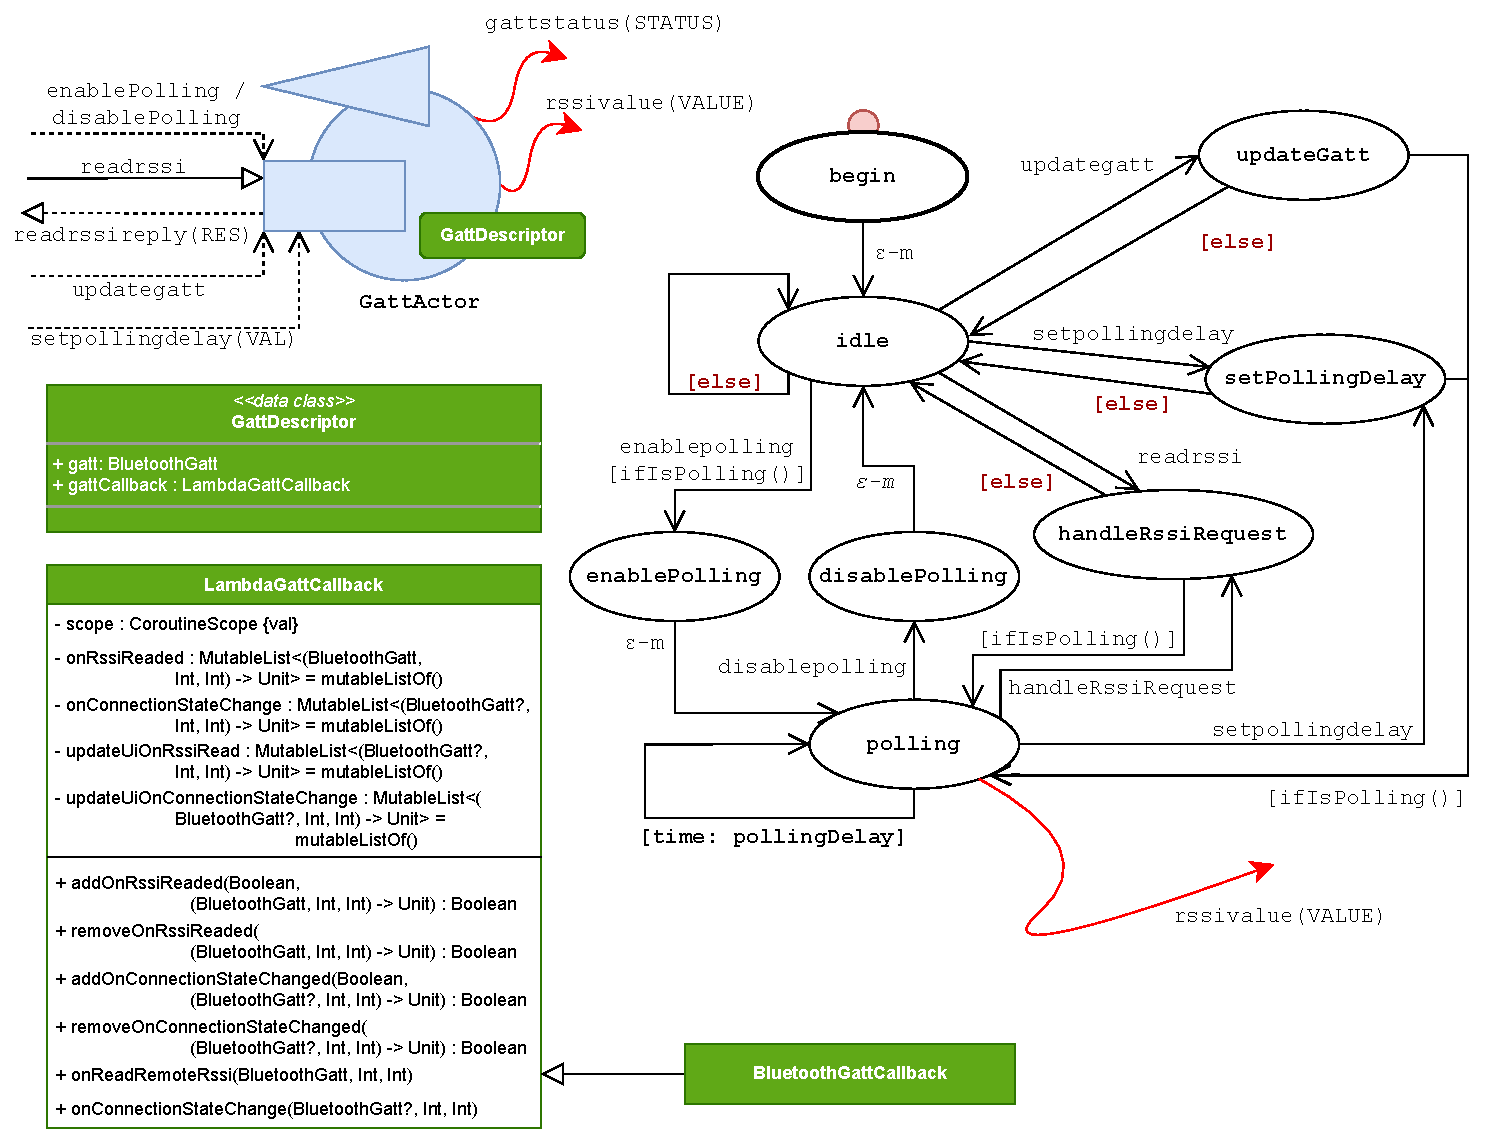
\includegraphics[width=\textwidth]{img/gattactor.pdf}
	\caption{State diagram of \texttt{GattActorActivity}}
	\label{fig:gattactor}
\end{figure}

The figure \ref{fig:gattactor} shows the state diagram of the \texttt{GattActor} and the \texttt{UML} of \texttt{GattDescriptor} class.

\textbf{Notice that the \texttt{GattActor} class has a \href{https://kotlinlang.org/docs/object-declarations.html\#companion-objects}{\texttt{companion object}} with an atomic variable that can be set in order to safely update the \texttt{GattDescriptor}.}

After the atomic variable is set, the actor can be \textit{notified} of this update by sending an \texttt{updategatt} dispatch.

About the states in \texttt{GattActor}:
\begin{itemize}
	\item \textbf{begin}:\\
	in this state the actor prepare itself for its job by taking the current \texttt{GattDescriptor} from the concurrent variable of the  companion object.
	
	\item \textbf{idle}:\\
	the actor simply waits for a command.
	
	\item \textbf{enablePolling}:\\
	the actor prepare itself to do polling work. After all is initialized, it automatically goes to \textbf{polling} state.
	
	\item \textbf{polling}:\\
	the actor perform the read of the \texttt{RSSI} value and then emits the proper event. After a time specified into \texttt{pollingDelay} variable, the actor returns in this state performing a new polling step.
	
	\item \textbf{disablePolling}:\\
	the actor prepare stop its polling job and returns to \texttt{idle} state.
	
	\item \textbf{setPollingDelay}:\\
	the actor updates the \texttt{pollingDelay} variable using the argument of the \texttt{setpollingdelay} message.
	
	\item \textbf{updategatt}:\\
	the actor updates its descriptor taking the current value using the companion object.
	
	\item \textbf{handleRssiRequest}:\\
	the actor handles a \texttt{readrssi} request by reading the current \texttt{RSSI} value and then sending a reply with the measurement.
	
\end{itemize}

\textbf{In the \texttt{updateGatt} state the actor automatically adds some callback to the \texttt{GATT} descriptor that emits the events when the \texttt{RSSI} value or \texttt{GATT} status is changed.} This because in \texttt{Android} the developer must register callbacks to the \texttt{BluetoothGatt} instance and that he has to ask for a reading (so the native mechanism is asynchronous).

\subsection{Project of positioning functionalities}

About positioning, as we studied in the course \texttt{Android} leaves to the developer only \textit{high-level} operations, hiding the lower levels.

So, the developer can only use a \textit{location provider} to notify his interest to monitor the position with no \textit{request/response} possibility. In addition, \texttt{Android} let the developer only to set some policies about precision, energy consumption, and so on and so forth.

\textbf{We need to have an high accuracy in order to send the proper command to the robot}, so we decide to use the \href{https://developers.google.com/android/reference/com/google/android/gms/location/FusedLocationProviderClient}{\texttt{FusedLocationProviderClient}} offered by the \textit{Gloogle Play Service API}.

\begin{figure}[h!]
	\centering
	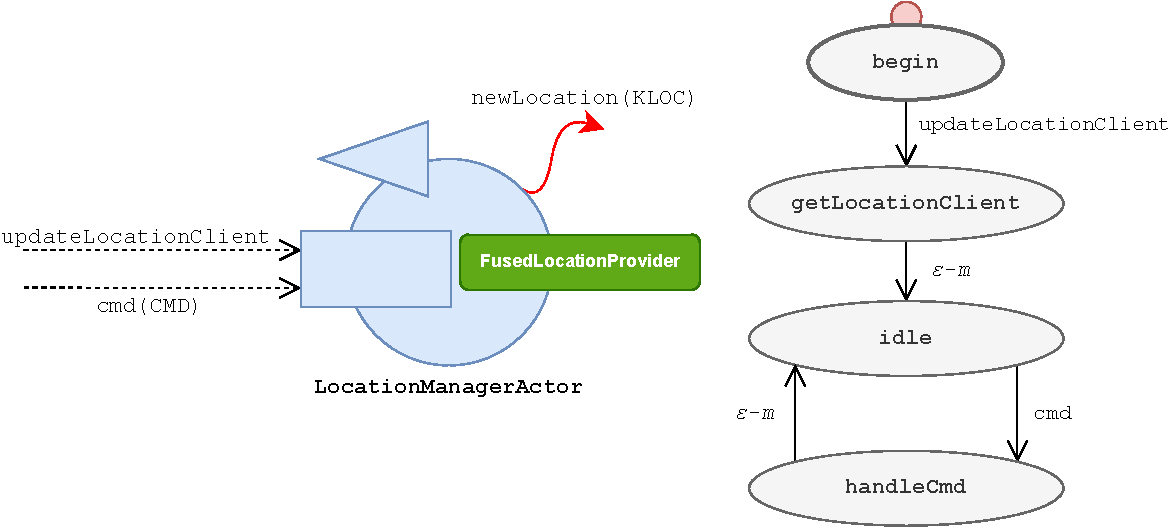
\includegraphics[width=\textwidth]{img/locationmanageractor.pdf}
	\caption{State diagram of \texttt{LocationManagerActor}}
	\label{fig:locationmanageractor}
\end{figure}

The figure \ref{fig:locationmanageractor} shows the state diagram of the actor that monitor the location.

About the states in \texttt{LocationManagerActor}:
\begin{itemize}
	\item \textbf{begin}:\\
	in this state the actor prepare itself for its job by taking the current \texttt{GattDescriptor} from the concurrent variable of the  companion object.
	
	\item \textbf{getLocationClient}:\\
	with a similar mechanism used by the \texttt{GattActor} with \texttt{GattDescriptor}, this actor retrieves the location provider \textbf{must have been previously set} by an activity. Then, the actor goes to \textbf{idle} state.
	
	\item \textbf{idle}:\\
	the actor waits for a command.
	
	\item \textbf{handleCmd}:\\
	the actor handle the dispatch that invites it to execute a command. Possible commands are two:
	\begin{itemize}
		\item \texttt{enableMonitoring}: set up the location provider in order to fire the \texttt{newLocation} event when the location is changed; as \texttt{Android} imposes, the used pattern implies callbacks automatically registered by the actor;
		
		\item \texttt{disableMonitoring}: stop the location provider work.
	\end{itemize}
	
\end{itemize}

\subsection{Project of \texttt{GitBertoActor}}

For time reasons, we will not provide details or graphs about the \texttt{GitBertoActor}.

\subsection{Project of the main activity}

We will not provide lots of details about the main activity that is \href{https://github.com/LucaLand/MobileSystemsProject-LL/blob/0.9.1/app/src/main/java/it/unibo/mobilesystems/MainMapsActivity.kt}{\texttt{MainMapsActivity}}.

This activity offers something similar to a \textit{navigator}: a map with a search box in which the user can type the desired address. The user can also tap a position on the map to set the target destination (following what the analyst said).

\begin{tcolorbox}
	\begin{center}
		\textbf{
			To manage map and calculate routes we decide to use a library called \href{https://github.com/osmdroid/osmdroid}{\texttt{OpenStreetMap}} with also some extensions from \href{https://github.com/MKergall/osmbonuspack}{\texttt{osmbonuspack}}.
			Then, in order to search addresses, to geocode them and to calculate path, we use the given \textit{API} using the \textit{ViewModel} pattern we have described.
		}
	\end{center}
\end{tcolorbox}

\begin{itemize}
	\item About \textbf{geocoding} we have created the classes \href{https://github.com/LucaLand/MobileSystemsProject-LL/blob/0.9.1/app/src/main/java/it/unibo/mobilesystems/geo/Geocoder.kt}{\texttt{Geocoder}} and \href{https://github.com/LucaLand/MobileSystemsProject-LL/blob/0.9.1/app/src/main/java/it/unibo/mobilesystems/geo/GeocoderViewModel.kt}{\texttt{GeocoderViewModel}}.
	
	\item About \textbf{path calculation} we have created the classes \href{https://github.com/LucaLand/MobileSystemsProject-LL/blob/0.9.1/app/src/main/java/it/unibo/mobilesystems/geo/PathCalculator.kt}{\texttt{PathCalculator}} and \href{https://github.com/LucaLand/MobileSystemsProject-LL/blob/0.9.1/app/src/main/java/it/unibo/mobilesystems/geo/PathViewModel.kt}{\texttt{PathViewModel}}
\end{itemize}

Then, the \texttt{MainMapsActivity} contains a map, an address box and a button to start the navigation process. When an address is written into the box, the \texttt{GeocoderViewModel} starts to search for the written address letting the user tap the desired and translating it into geographical coordinates.
So, when the user clicks on the start button, the \texttt{PathViewModel} calculates the path and the navigation is started by \textbf{sending proper messages to the business actor} we have presented.

